\documentclass[../DefinizioneDiProdotto.tex,lanscape]{subfiles}
\begin{document}

\section{Diagrammi riassuntivi package}
	Di seguito sono riportati tutti i package dell'applicativo per chiarire la relazione tra le componenti e le classi al suo interno visto l'utilizzo del pattern MVP. Per chiarezza ed esigenza di spazio le classi rappresentate all'interno dei package sono rappresentate senza metodi e attributi.


\begin{figure}[H]
	%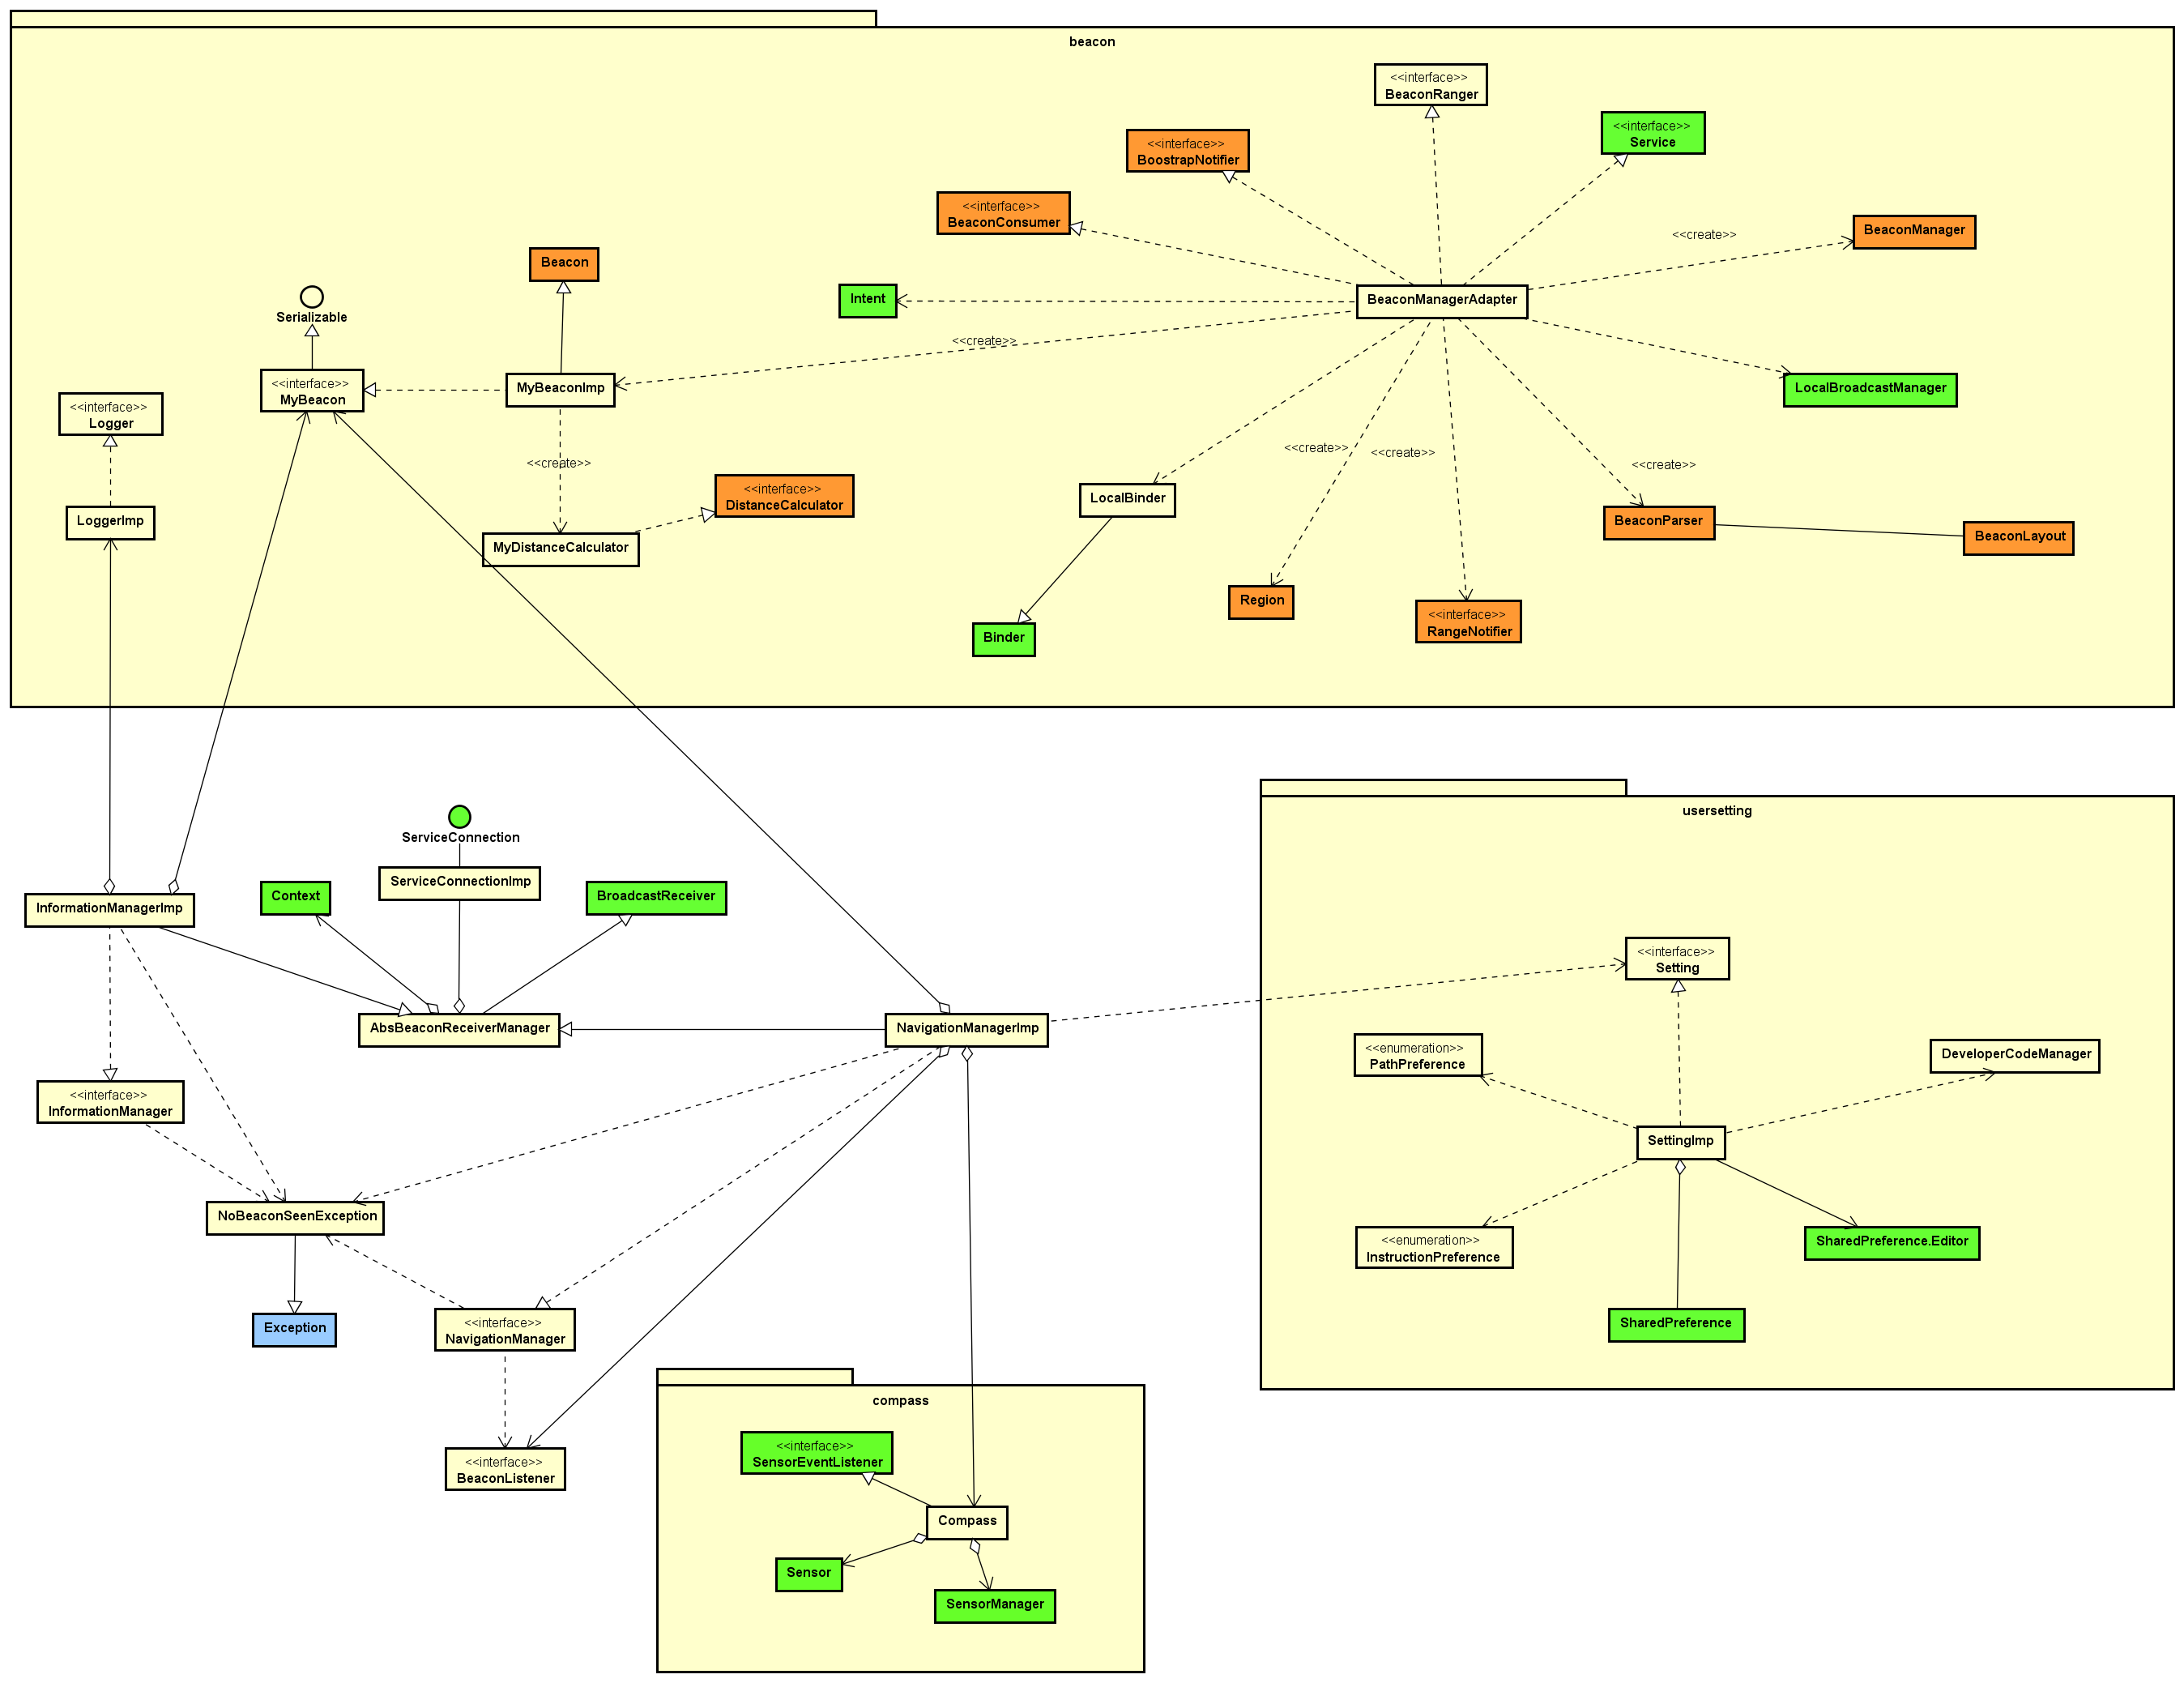
\includegraphics[angle=90,width=\textwidth, height=\textheight, keepaspectratio]{diagrams/ModelCompleteNoMethods/PNGpackage/model}
	\label{modelPackage}
	\caption{Diagramma delle classi - model}
\end{figure}

\begin{figure}[H]
	%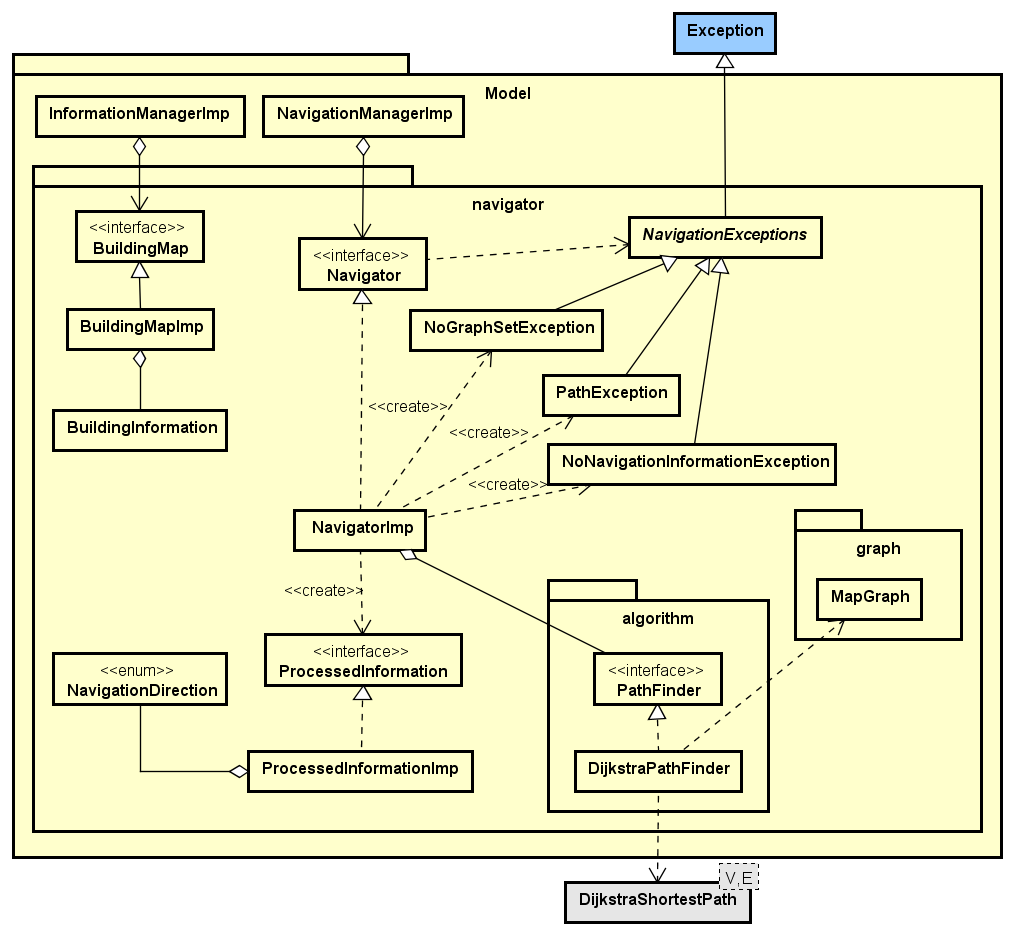
\includegraphics[angle=90,width=\textwidth,, height=580pt, keepaspectratio]{diagrams/ModelCompleteNoMethods/PNGpackage/navigator}
	\label{navigatorPackage}
	\caption{Diagramma delle classi - model::navigator}
\end{figure}

\begin{figure}[H]
	%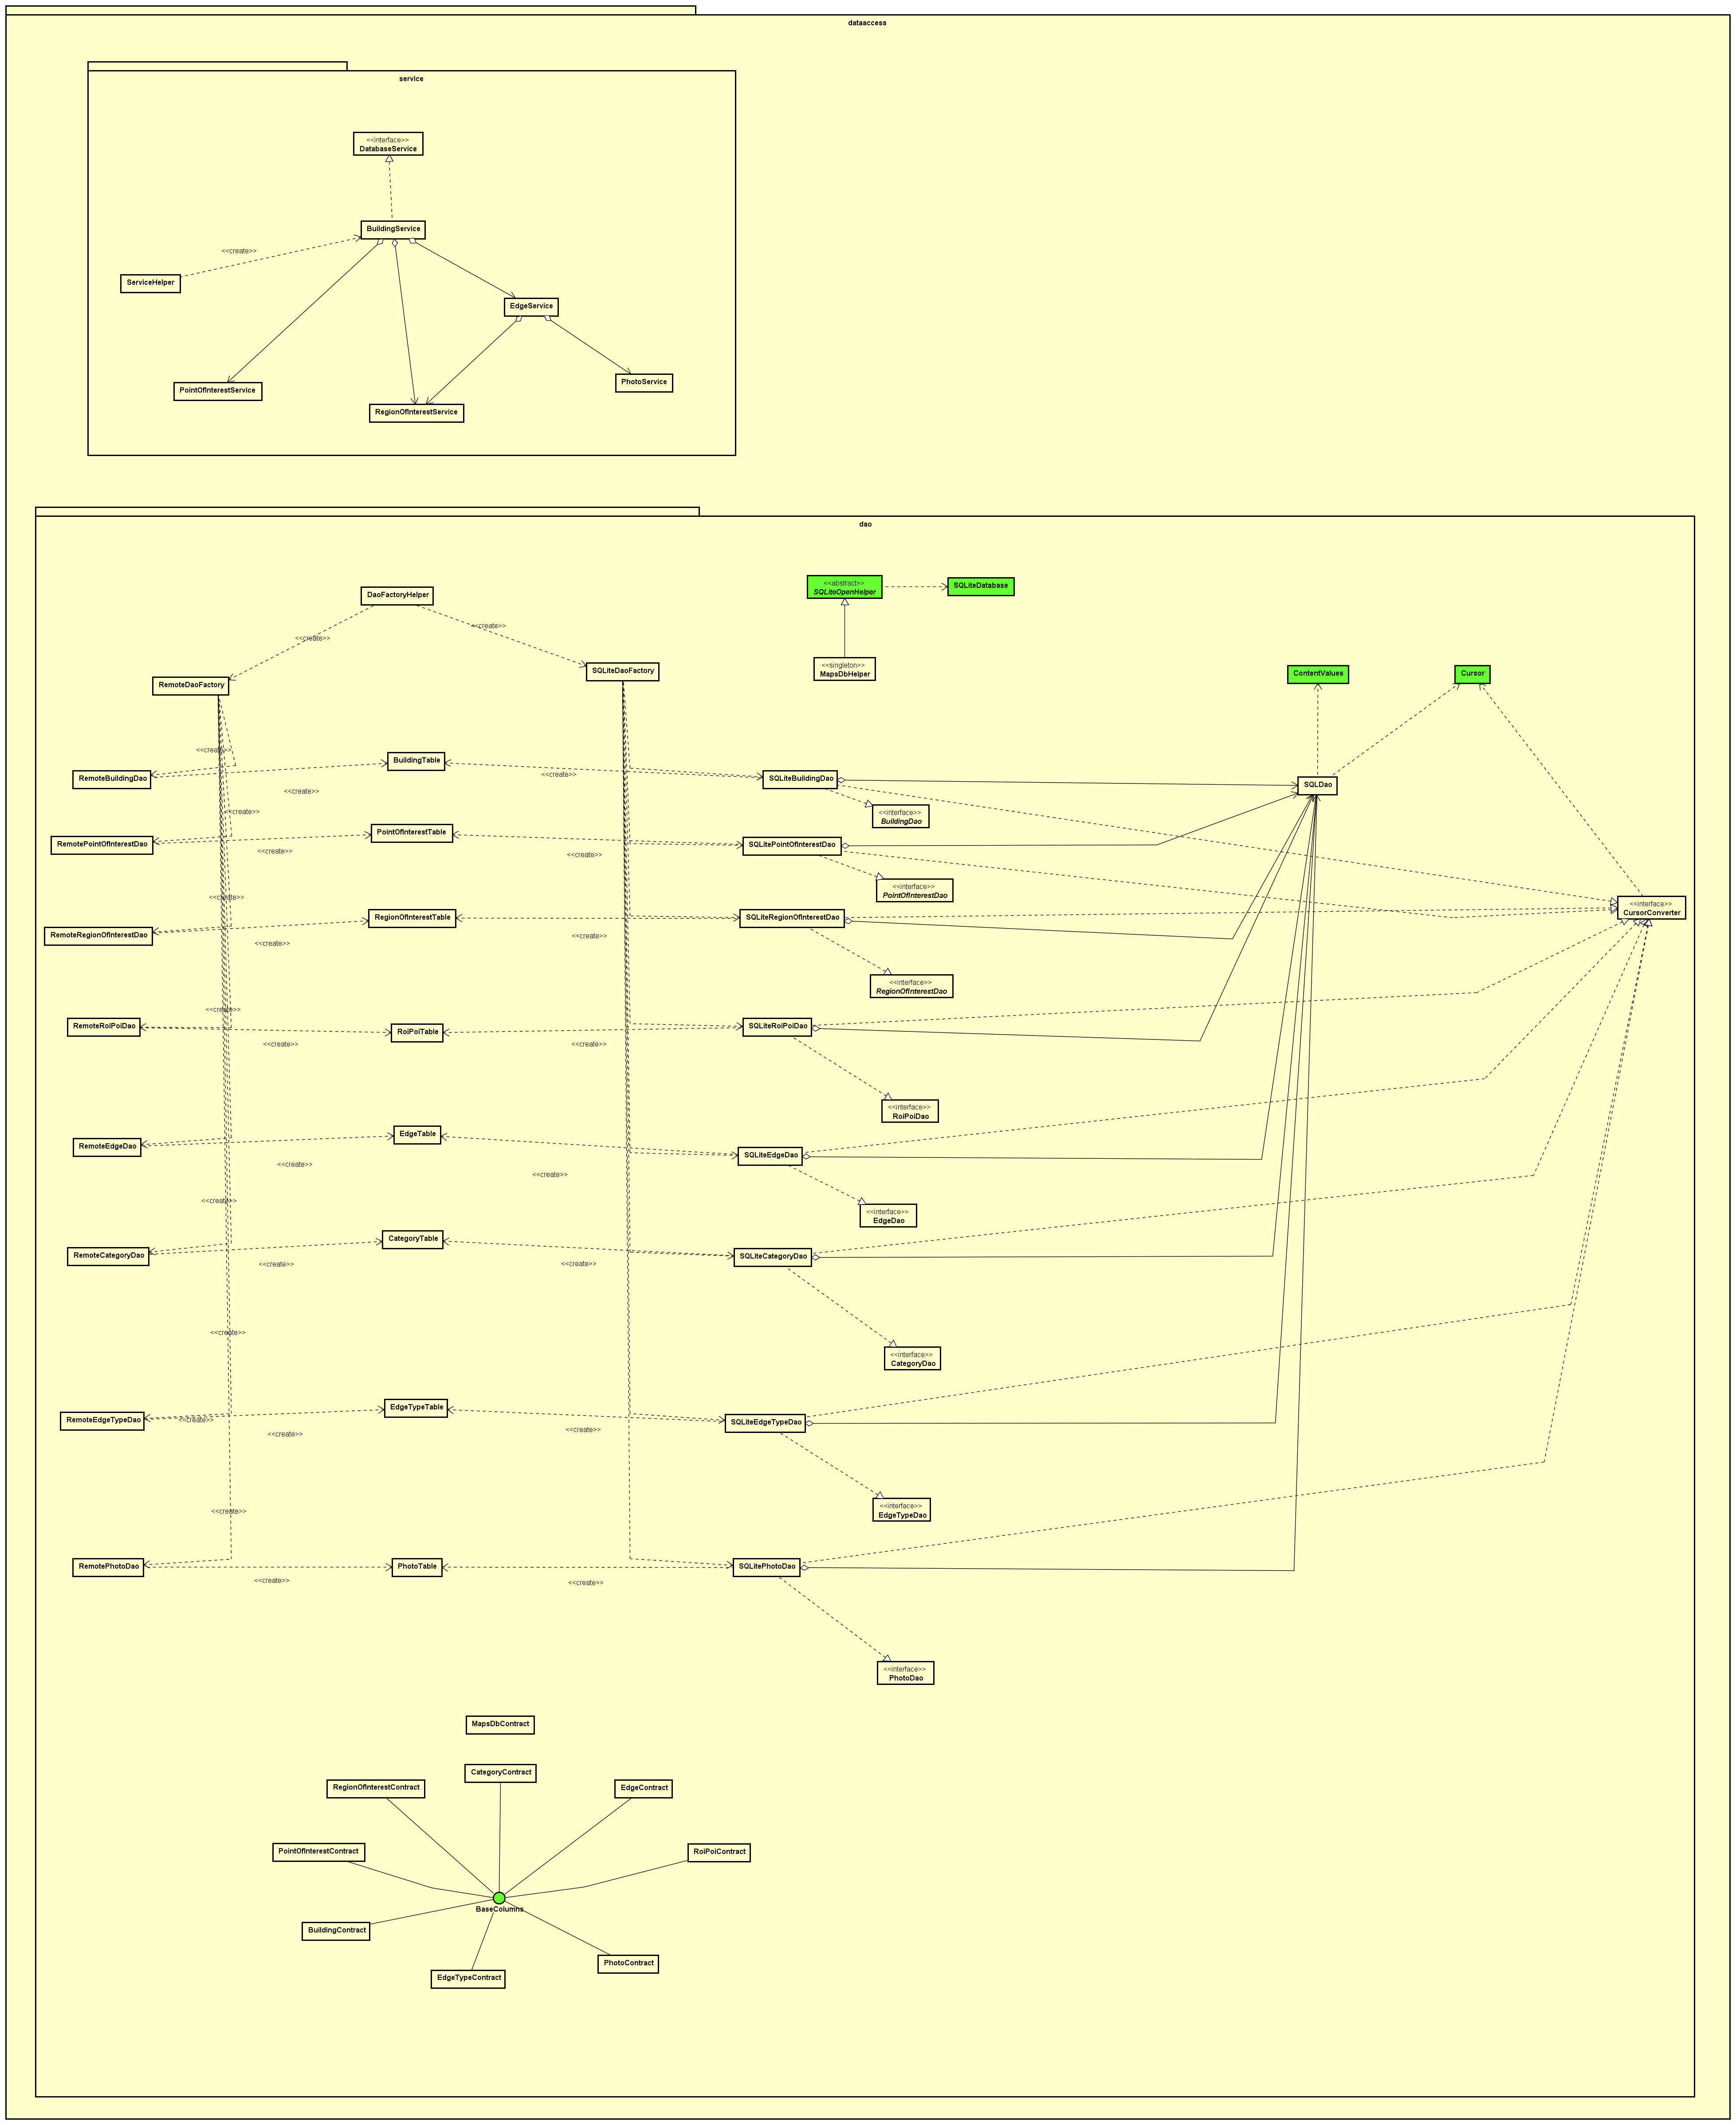
\includegraphics[width=\textwidth]{diagrams/ModelCompleteNoMethods/PNGpackage/dataaccess}
	\label{dataaccessPackage}
	\caption{Diagramma delle classi - model::dataaccess}
\end{figure}

\begin{figure}[H]
	%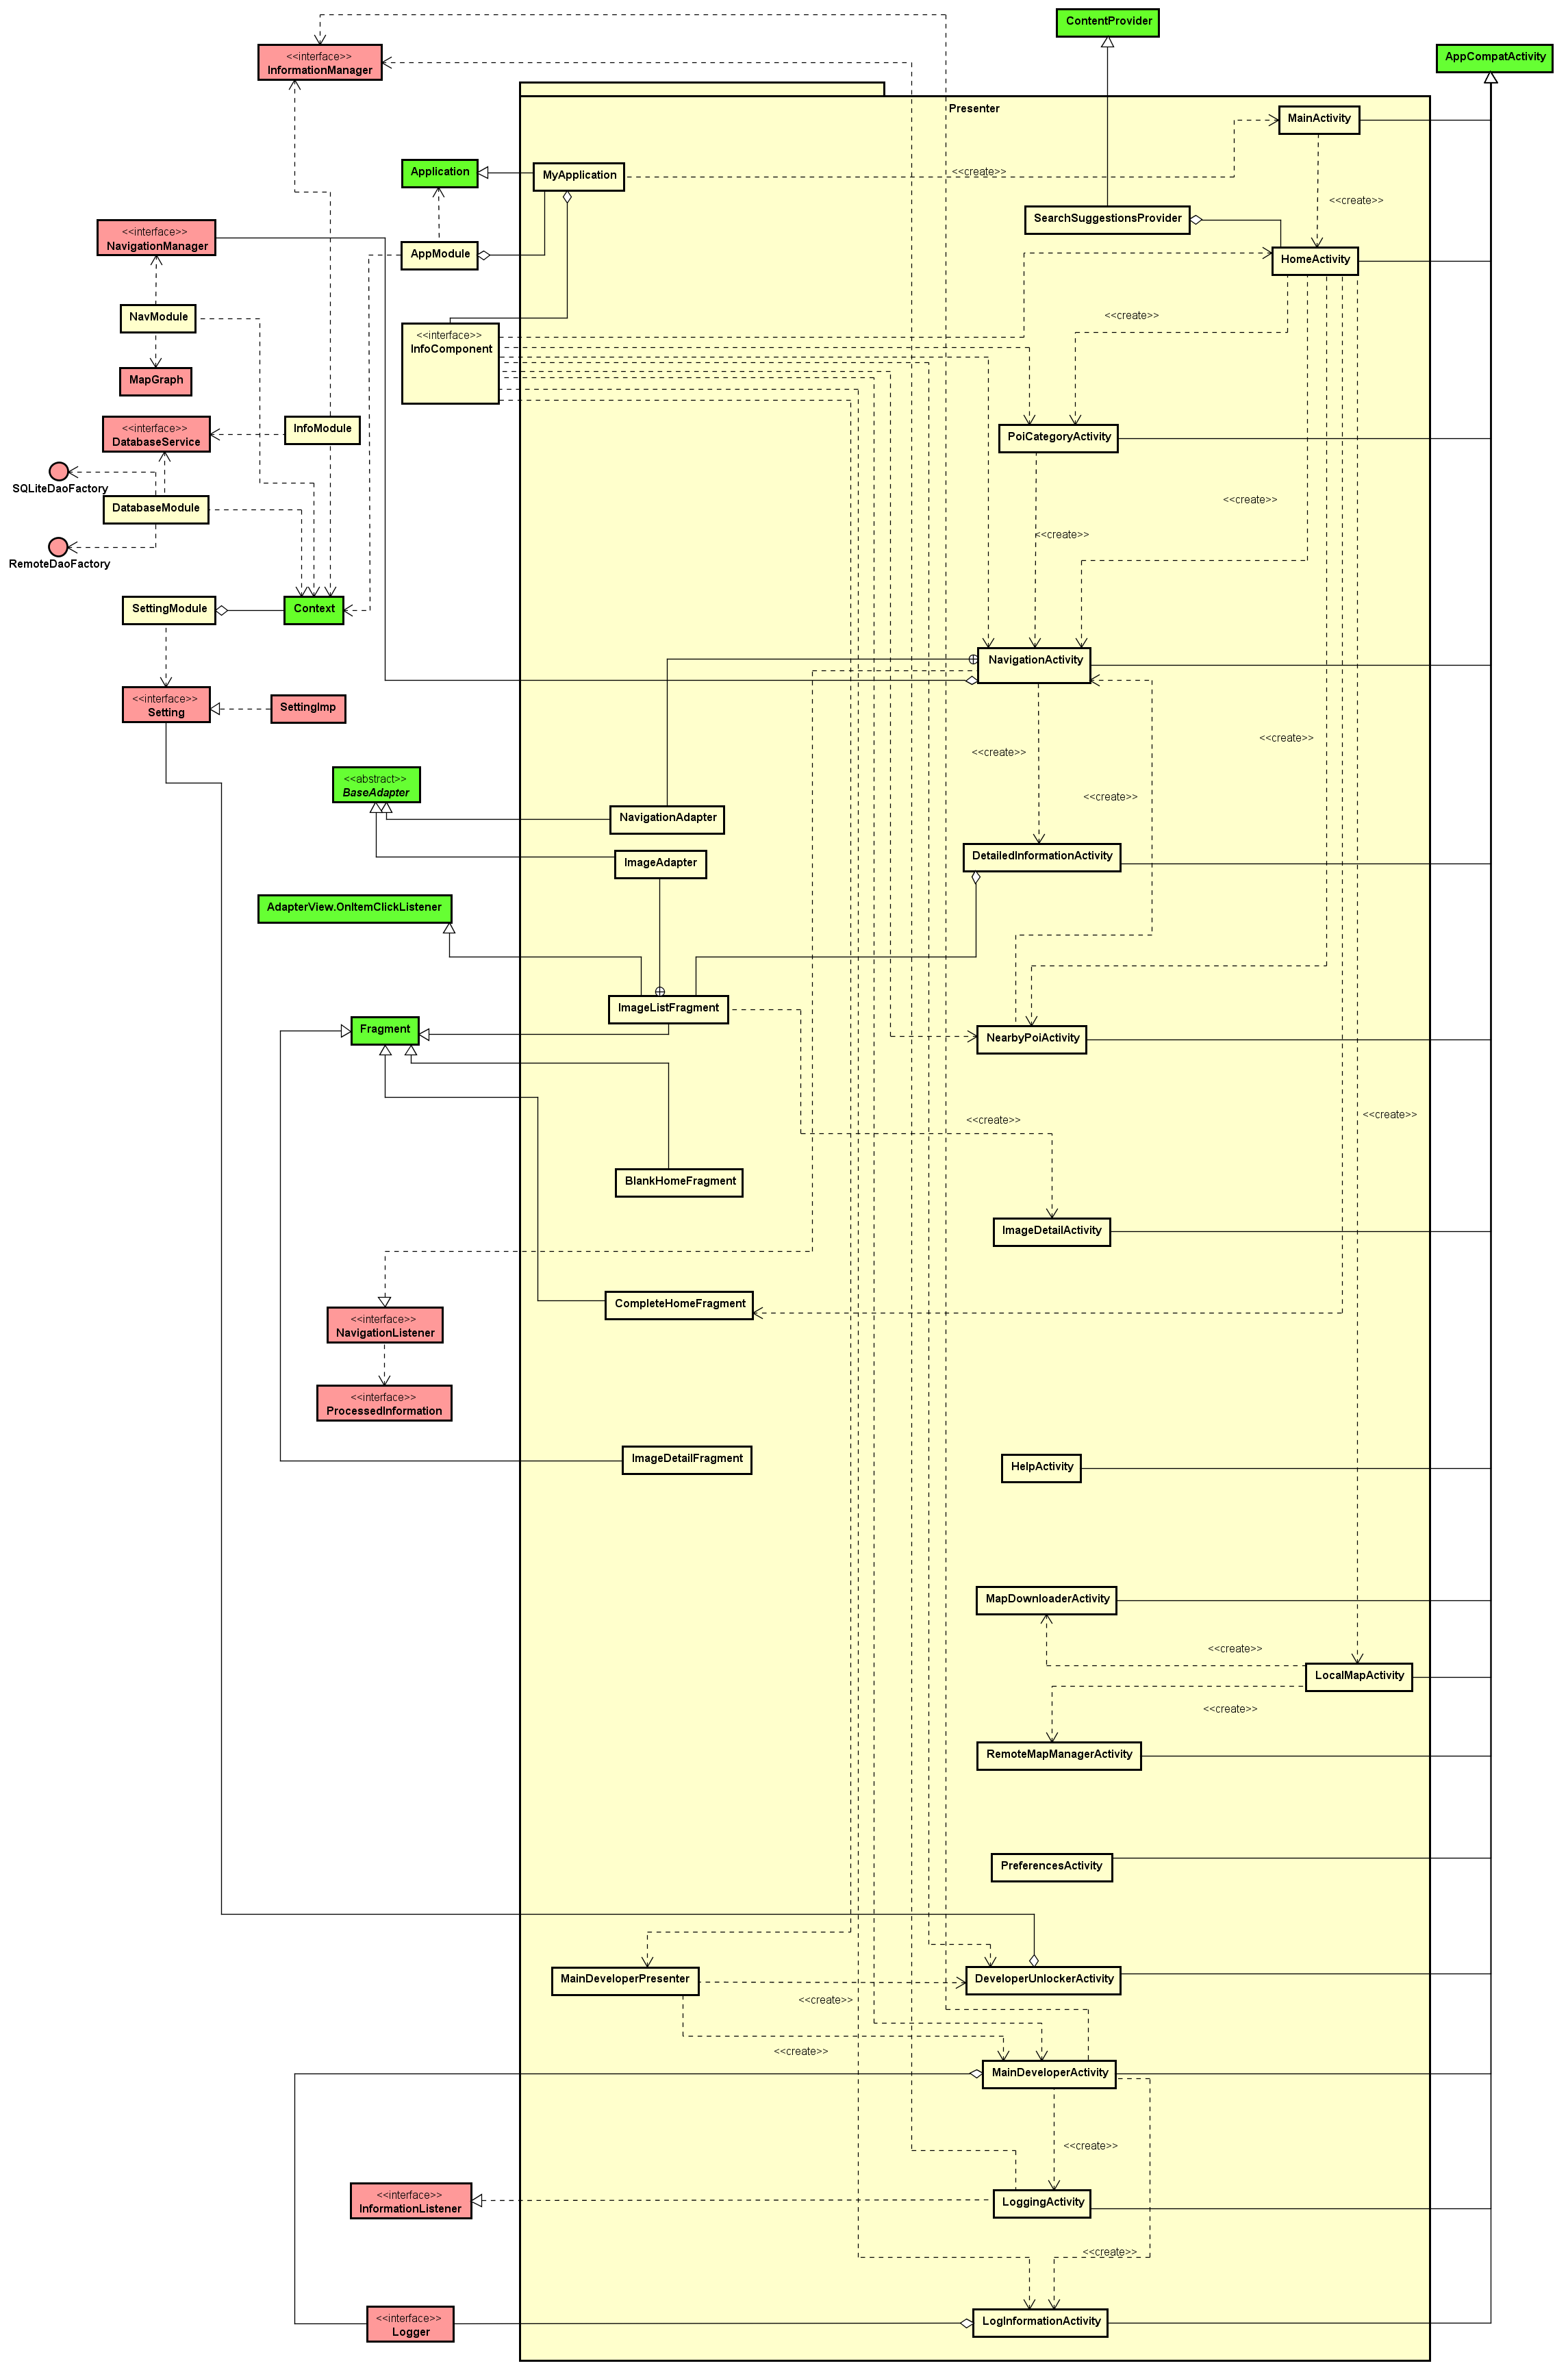
\includegraphics[width=\textwidth, height=19cm]{diagrams/ModelCompleteNoMethods/PNGpackage/presenter}
	\label{presenterPackage}
	\caption{Diagramma delle classi - presenter}
\end{figure}

\begin{figure}[H]
	\centering
	%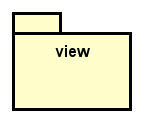
\includegraphics[height=20cm]{diagrams/ModelCompleteNoMethods/PNGpackage/view}
	\label{viewPackage}
	\caption{Diagramma delle classi - view}
\end{figure}

\begin{figure}[H]
	\centering
	%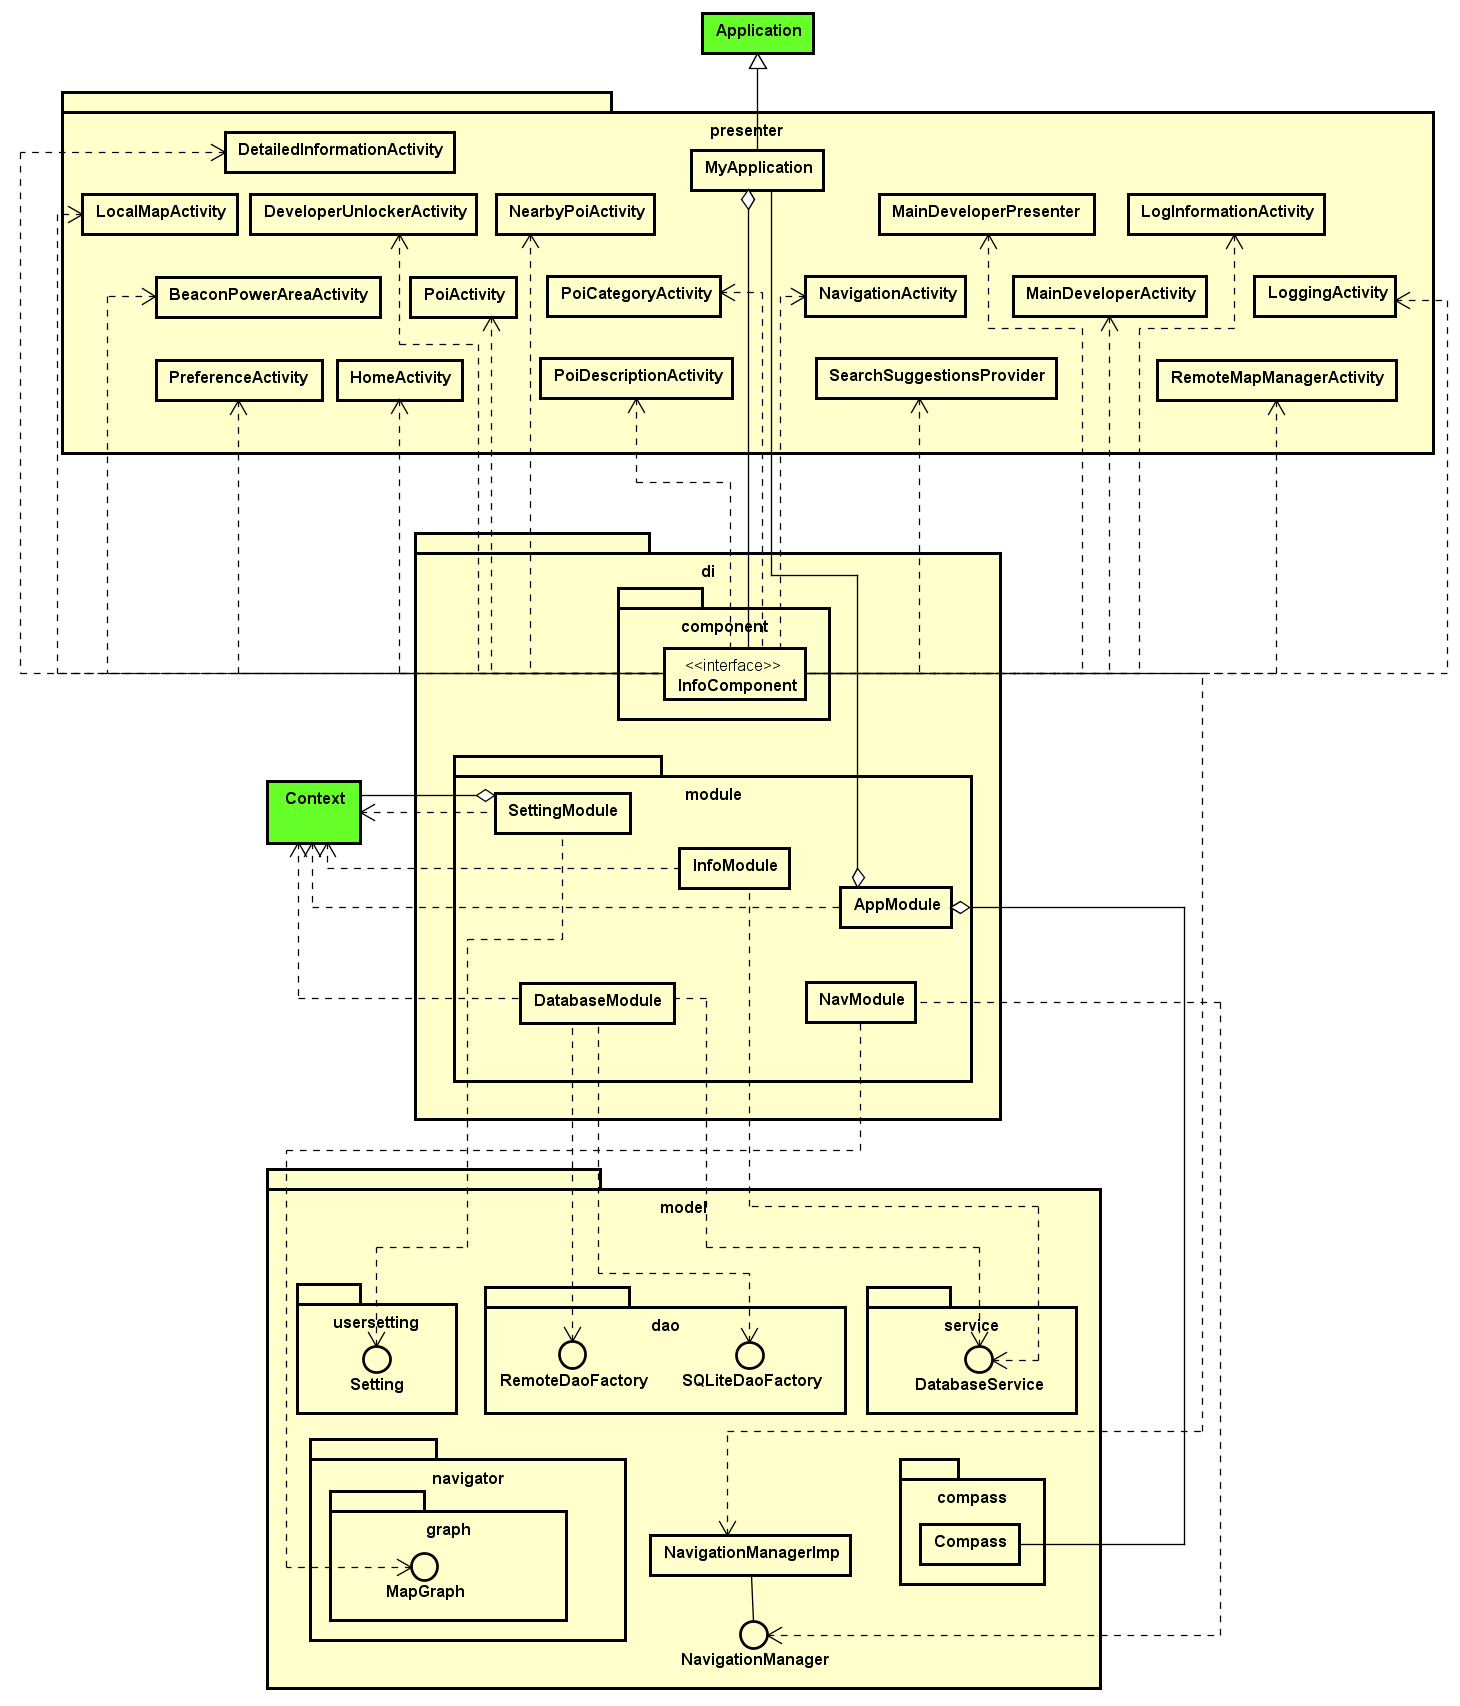
\includegraphics[height=19cm,width=\textwidth]{diagrams/ModelCompleteNoMethods/PNGpackage/di}
	\label{diPackage}
	\caption{Diagramma delle classi - dependency injection}
\end{figure}

\end{document}